本章では、VDMを如何に導入し、どのような開発方法・体制を採用したかを述べる。

\section{VDMの教育}
	\label{Education}
	\index{VDMのきょういく@VDMの教育}

	日本でVDMの導入に成功した表\ref{VDMeffectTable}の事例で行われた教育の内容を表\ref{VDMEducation}に示す。

\begin{table}[h]
	\caption[VDMの教育]{VDMの教育}
	\index{VDMのきょういく@VDMの教育}
	\label{VDMEducation}
	\begin{center}
		\setlength{\tabcolsep}{3pt}
		\begin{tabular}{|p{11zw}|p{5zw}|p{4zw}|p{10zw}|p{9zw}|p{12zw}|} \hline
			組織 & セミナー & 教材 & コンサルティング & 受講者 & 備考 \\ \hline\hline

			日本フィッツ & 4日間 & 英語 & 
				形式手法知識を持った要員とオブジェクト指向分析・設計手法(OOA/OOD)専門家の要員が相談 & 
				平均年齢50歳弱 & VDM記述予定者の3分の1(2人)は英語で脱落 \\ 
				(現SCSK) & & & & 形式手法知識4人有 & \\ 
				 &  & & & ソフト工学知識有 & C++, Java, 形式手法について、実践経験無 \\ 
				 &  & & & 業務知識無 & \\ \hline

			フェリカネットワークス & 4日間 &  日本語 & 3ヶ月/週1回 & 平均年齢20歳代 & \\ 
				 & & & & 形式手法知識無 & \\ 
				 & & & & ソフト工学知識無 & \\ 
				 & & & & 業務知識有 & \\ \hline
			産業技術総合研究所 & 無し & 日本語 & 最初は無し & 平均年齢30歳代 & 周囲に形式手法経験者多数 \\ 
				オムロン & 自習 & 参考文献 \cite{Sakoh2010} \cite{Sahara2008} & その後、3ヶ月/週1回 & 形式手法知識1人有 & \\ 
				 & & & & ソフト工学知識無 & \\ \hline
		\end{tabular}
	\end{center}
\end{table}

海外の形式手法使用事例でも、形式手法の初期教育は約1週間であり、
その後3ヶ月ほど形式手法の専門家によるコンサルティングを経て、
成功している事例がほとんどであり\cite{SEC2012FMREPORT}、
日本での成功例の場合と教育方法・手順はほとんど同じである。

なお、日本フィッツの場合は開発チーム全員がVDMセミナーを受講したが、
フェリカネットワークスは仕様記述フレームワーク作成予定者のみVDMセミナーを受講した。

\section{仕様記述}
	\label{Specification}
	\index{しようきじゅつ@仕様記述}

	VDM++を使って、仕様記述者がそれぞれ独自の仕様記述を行った場合、
	仕様の可読性や再利用性、保守性などが損なわれることが予想されたので、
	仕様記述のフレームワークを定め、仕様ライブラリを作成した。

\subsection{仕様記述フレームワーク}
	\label{SpecFramework}
	\index{しようふれーむわーく@仕様記述フレームワーク}

仕様記述フレームワークは、仕様のどの部分に何を書くかを定めた規則である。
どのように書くかを示すテンプレートとして提示したり、
関連する仕様ライブラリを使用するよう指示する部分もあるが、
多くは、日本語文で定めた規則である。

仕様記述のためのフレームワークを作成した目的は以下の通りである。

	\begin{itemize}
	\item 仕様の可読性、再利用性、保守性の向上
	\item 仕様記述者のVDM技術レベルと仕様の階層を対応させ、VDM初級者でも仕様記述を行えるようにする
	\item DBインターフェースの隠蔽を行い、RDBによる実装を行いやすくする(日本フィッツ事例(\ref{JFITS}節)の場合)
	\item 実装側フレームワークと対応させ、仕様とプログラムの対応関係が分かりやすいようにする(日本フィッツ事例の場合)
	\end{itemize}

\subsubsection{仕様記述フレームワークの概要}
	\index{しようふれーむわーくのがいよう@仕様記述フレームワークの概要}

	\paragraph{仕様記述の対象}
		\index{しようきじゅつのたいしょう@GUIの捨象}

	日本フィッツ事例(\ref{JFITS}節)では、ユースケース・レベルの業務論理(Business Logic)を仕様記述の対象とした。
	
	フェリカネットワークス事例(\ref{FeliCa}節)では、ファームウェアのAPI仕様を仕様記述の対象とした。

	\paragraph{GUIの捨象}
		\index{GUIのしゃしょう@GUIの捨象}
	仕様記述フレームワーク作成では、GUIは捨象して記述しなかった。

	これは、日本フィッツ事例の場合、サーバー側のユースケース・レベルの仕様を記述することが一番重要であり、
	クライアント側のGUIは、ユースケース・レベルの仕様記述とかなりの部分が重複するため、
	従来通りの画面仕様を中心とした仕様を使った。

	GUIを除くクライアント側の仕様も、記述するための仕様記述フレームワークは試作したが、
	サーバー側のユースケース・レベル仕様との重複が多く、記述工数と比較して効果が薄いと判断し、
	記述しなかった。
	
	フェリカネットワークス事例の場合、仕様記述対象がファームウェアのAPI仕様であったため、
	そもそも、GUI部分は無かった。

	\paragraph{仕様記述フレームワークの具体例}
		\index{しようふれーむわーくのぐたいれい@仕様記述フレームワークの具体例}

	日本フィッツ事例(\ref{JFITS}節)の仕様記述フレームワークを、表\ref{SpecFrameJFITS}に示す。

\begin{table}[h]
	\caption[仕様記述フレームワーク(日本フィッツ)]{仕様記述フレームワーク(日本フィッツ)}
	\index{しようふれーむわーくにほんふぃっつ@仕様記述フレームワーク(日本フィッツ)}
	\label{SpecFrameJFITS}
	\begin{center}
		\setlength{\tabcolsep}{3pt}
		\begin{tabular}{|l|l|l|} \hline
			仕様記述の階層 & 充足する記述領域 & 必要なVDM技量  \\ \hline\hline
			テストケース  & 回帰テスト & 初級 \\ \hline
			シナリオ  & 事後条件記述 & 初級 \\ \hline
			業務論理  & 業務アプリケーション & 初級 \\ \hline
			要求辞書  & 業務知識兼用語辞書 & 中級 \\ \hline
			仮想DBアクセス応用  & DB登録、抽出、削除、訂正 & 上級 \\ \hline
			仮想DBアクセス基本  & undo, old valueアクセス, 差分 & 上級 \\ \hline
			基本レコード構造  & 必要データ & 初級 \\ \hline
		\end{tabular}
	\end{center}
\end{table}

	この表で、シナリオ階層を作ったのは、
		\index{しなりおかいそう@シナリオ階層}
	業務論理で事後条件記述を試みた所、200行〜300行の事後条件となってしまい、
	可読性や保守性に問題があると判断したためである。
	例えば、「口座を解説する」といった一つの業務論理に、
	「個人顧客の口座を開設するシナリオ」「法人顧客の口座を開設するシナリオ」「口座開設が失敗するシナリオ」といったように、
	複数のシナリオを想定し、それぞれに事後条件を記述することで、
	各シナリオは20行〜30行程度の事後条件となり、読みやすくなった。
	したがって、シナリオ階層を設定した場合は、業務論理階層に事後条件は記述しない。

	業務論理とシナリオとテストケースの対応関係を図\ref{fig:SpecTree}に示す。

\begin{figure}[h]
	\centering
	{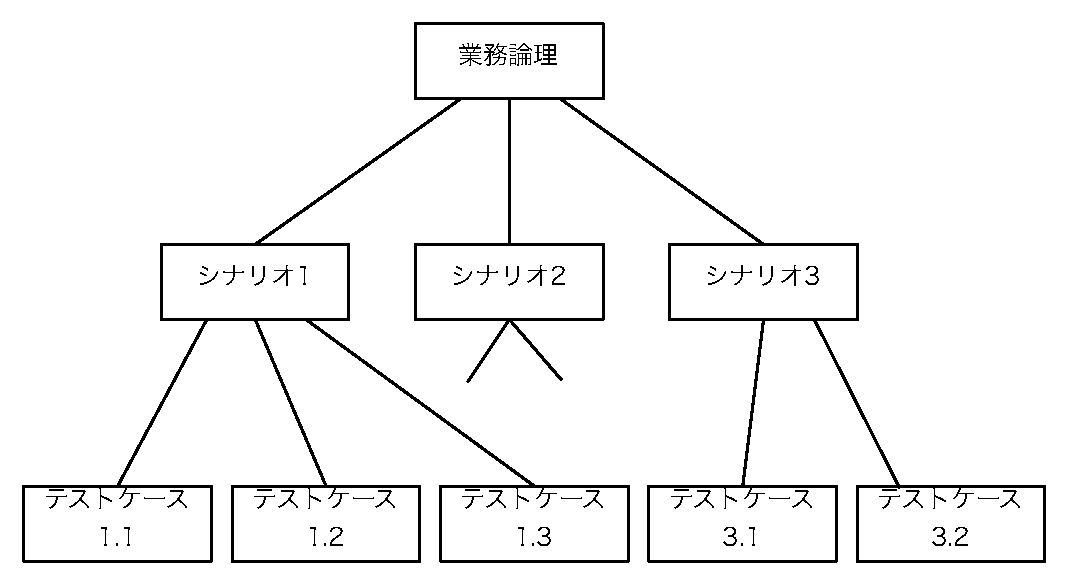
\includegraphics[width=55zw, keepaspectratio]{./Chapter4/image/SpecTree.pdf}}
	\caption{業務論理とシナリオとテストケースの対応関係}
	\label{fig:SpecTree}
	\index{ぎょうむろんりとてすとけーすのたいおうかんけい@業務論理とシナリオとテストケースの対応関係}
\end{figure}


	要求辞書階層は、業務論理階層で使う用語を定義している。
		\index{ようきゅうじしょかいそう@要求辞書階層}
	この階層では、名詞に対応するクラス名や型名だけでなく、
	動詞に対応する関数(function)や操作(operation)も記述する。
	この階層に記述される仕様は、いわゆる暗黙知の明示的な仕様となるため、
		\index{あんもくち@暗黙知}
	何を記述すべきかも含めて、記述は容易ではないが、この階層が記述できることにより、
	暗黙知を明示的な知識として共有することができるようになる。
	したがって、要求辞書階層の再利用性は、同じ問題領域であれば、かなり高い。
	要求辞書階層を記述する仕様記述者は、VDM++の構文をある程度マスターしていなければならない。

	\ref{FareModel}章で紹介する運賃計算モデルの仕様記述フレームワークを、表\ref{SpecFrameFare}に示す。

\begin{table}[h]
	\caption[仕様記述フレームワーク(フェリカネットワークス)]{仕様記述フレームワーク(運賃計算モデル)}
	\index{しようふれーむわーくうんちんけいさんもでる@仕様記述フレームワーク(運賃計算モデル)}
	\label{SpecFrameFare}
	\begin{center}
		\setlength{\tabcolsep}{3pt}
		\begin{tabular}{|l|l|l|} \hline
			仕様記述の階層 & 充足する記述領域 & 必要なVDM技量  \\ \hline\hline
			テストケース  & 回帰テスト & 初級 \\ \hline
			業務論理  & 業務アプリケーション & 初級 \\ \hline
			要求辞書  & 業務知識兼用語辞書 & 中級 \\ \hline
			ユーティリティ  & 共通機能 & 上級 \\ \hline
		\end{tabular}
	\end{center}
\end{table}

	この運賃モデルは、教育用に基本的な機能だけを持った仕様を記述しているため、
	仕様記述フレームワークの階層も深くはない。

	ユーティリティ階層は、鉄道ネットワークのグラフ構造から最短距離を計算する
	ダイクストラ算法のために作った。
	当然ながら、ユーティリティ階層の再利用性は、要求辞書階層よりも更に高い。

	図\ref{fig:ClassDiagram4Fare}に、
	運賃計算モデルのクラス図と、仕様記述フレームワーク階層の対応関係を示す。

\begin{figure}[h]
	\centering
	{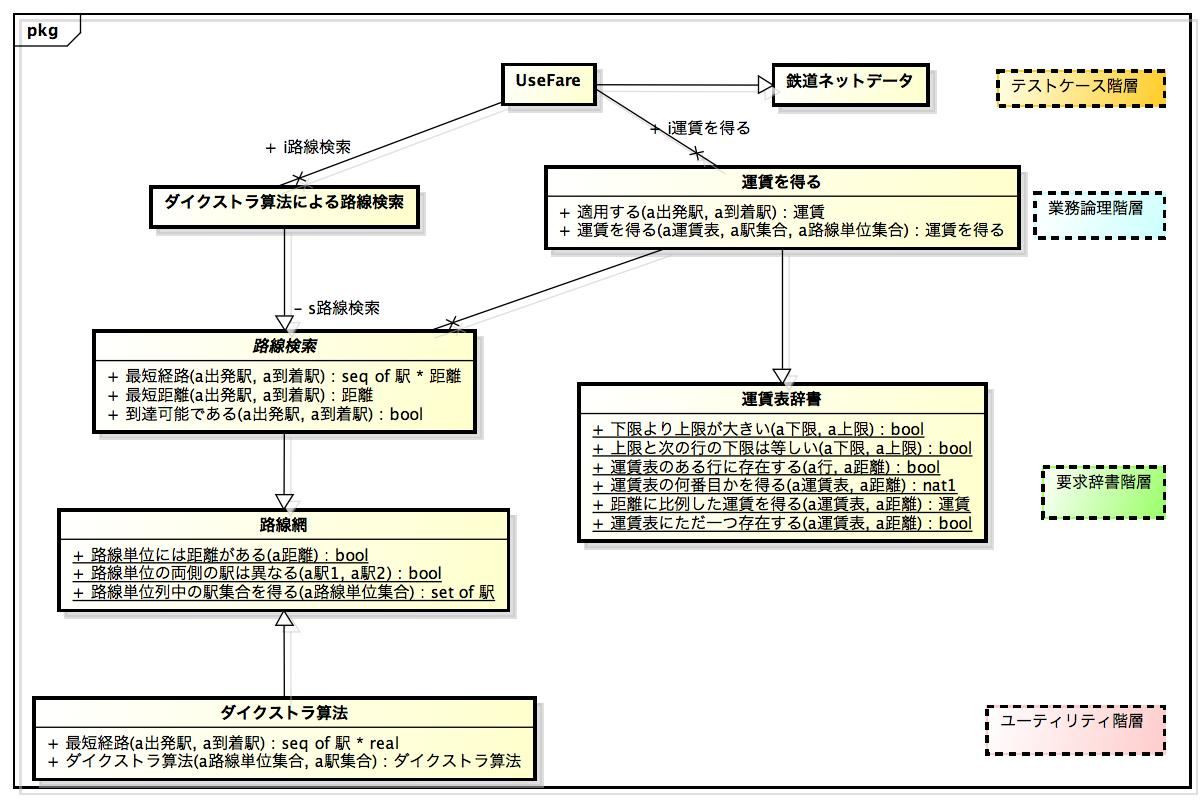
\includegraphics[width=55zw, keepaspectratio]{./Fare/image/ClassDiagram.jpg}}
	\caption{運賃計算モデルのクラス図}
	\label{fig:ClassDiagram4Fare}
	\index{うんちんけいさんもでるのくらすず@運賃計算モデルのクラス図}
\end{figure}

	仕様記述フレームワークの各階層の具体例については、\ref{FareModel}章を参照していただきたい。

\subsection{仕様ライブラリ}
	\label{SpecLibrary}
	\index{しようらいぶらり@仕様ライブラリ}

	以下のライブラリ3000行ほどを、あらかじめ作成した。

	\begin{itemize}
	\item 文字、文字列ライブラリ \\
		VDM++は、特定の文字コードに依存しないよう、文字、文字列順という概念がないが、
		エンタープライズ系のシステムではソート順として多用されるため。
	\item 暦、日時、期間ライブラリ \\
		エンタープライズ系のシステムでは、暦、日時、期間などに関する欠陥が多いため。
	\item 列ライブラリ \\
		エンタープライズ系のシステムでは、合計、平均、ソートなどが多用されるため。
	\item 待ち行列、ハッシュ表ライブラリ \\
		データ構造としてよく使われるため。
	\item 数値計算関連ライブラリ \\
		実数の桁数、微分、ニュートン法などを使うことが予想されたため。
	\item その他、業務に関連したライブラリ
	\end{itemize}

\section{仕様テスト}
	\label{SpecTest}
	\index{しようてすと@仕様テスト}

	仕様のテストは、以下のようにして行った
	\footnote{詳細については、VDMTools ユーザマニュアル(VDM++) 2.0
		{\url{http://www.vdmtools.jp/modules/tinyd2/index.php?id=2}}
	を参照のこと}
	。

	\begin{itemize}
	\item VDMToolsで、静的チェック
		\begin{itemize}
		\item 構文チェック、型チェック \\
			\index{こうぶんちぇっく@構文チェック}
			\index{かたちぇっく@型チェック}
			型チェックは、当初予想していたより、はるかに多くの単純ミスを発見した。
		\item 証明課題生成を行ってレビュー \\
			\index{しょうめいかだいせいせい@証明課題生成}
			事前条件の記述忘れを、かなりの確率で発見できた。
		\end{itemize} 
	\item VDMToolsで、動的チェック \\
		\index{どうてきちぇっく@動的チェック}
		VDM++インタープリタとデバッガで実行可能仕様
		\index{じっこうかのうしよう@実行可能仕様}
		\footnote{陽仕様とも言う}
		をテストした。
		\begin{itemize}
		\item 動的に、不変条件・事前条件・事後条件をチェック
			\index{ふへんじょうけん@不変条件}\index{じぜんじょうけん@事前条件}\index{じごじょうけん@事後条件}
		\item 組合せテスト機能を利用して、組合せテスト(\ref{CombinatorialTest}参照)を実行
			\index{くみあわせきのう@組合せテスト機能}
		\item 回帰テスト支援ライブラリを改良して回帰テスト(\ref{RegressionTest}参照)を実行 \\
				\index{かいきてすと@回帰テスト}
				回帰テストケースを作成するのはそれなりに大変だが、仕様修正に対して非常に効果があった。
		\item コードカバレージ(網羅性検査)機能で、テスト達成率を測定 \\
				\index{こーどかばれーじ@コードカバレージ}\index{もうらせいけんさ@網羅性検査}
				C0(命令)レベルで、
				85\%(フェリカネットワークス事例(\ref{FeliCa}節))から95\%(日本フィッツ事例(\ref{JFITS}節))を達成した。
		\item 検出した矛盾点を、要求仕様に反映
		\end{itemize} 
	\item VDM仕様に基づいて、ランダム評価ツールを作成し、
			数億件のテストケースを生成し、動的チェック(フェリカネットワークス事例)を行った。
		\begin{itemize}
		\item 仕様エミュレータを内蔵
		\item 実装に対し、ランダムにコマンドを送信し、応答が正しいか確認
		\end{itemize} 
	\end{itemize} 

\subsection{組合せテスト}
	\label{CombinatorialTest}
	\index{くみあわせてすと@組合せテスト}

	組合せテスト(Combinatorial Test)は、指定したテストパターンから、テストケースの組合せを生成し、テストする。
	テストでエラーになったものと同じパターンのテストケースは実行せず、テストの実行効率を上げる。

	下記の例のように、trace句の後に組合せテストケースを記述する。
	各組合せテストケースはラベル(今の場合S1, S2など)で始まり、
	VDMの構文の後ろに組合せの正規表現記述を行う。
		\index{せいきひょうげんきじゅつ@正規表現記述}
	正規表現記述の説明は、VDM++の注釈として示した。

\begin{verbatim}
class UseUniqueNumber
instance variables
sUN : 発番者 :=  new 発番者();

traces
S1 :  let n in set {1,2,3,4} in sUN.発番する(n){10,12}   -- 10回から12回繰り返す

S2 :  let n in set {2} in sUN.発番する(n)+   -- 1回から既定回数繰り返す

S3 :  let n in set {3} in sUN.発番する(n)*   -- 0回から既定回数繰り返す

S4 :  let n in set {4} in sUN.発番する(n){10002}   --10002回繰り返す

end UseUniqueNumber
\end{verbatim}

図\ref{fig:CombinatorialTestScreen}に、組合せテスト実行後のOverture tool画面例を示す
\footnote{VDMToolsは、組合せテスト実行結果をインタープリタ・ウィンドウにログとして表示する}。

\begin{figure}[h]
	\centering
	{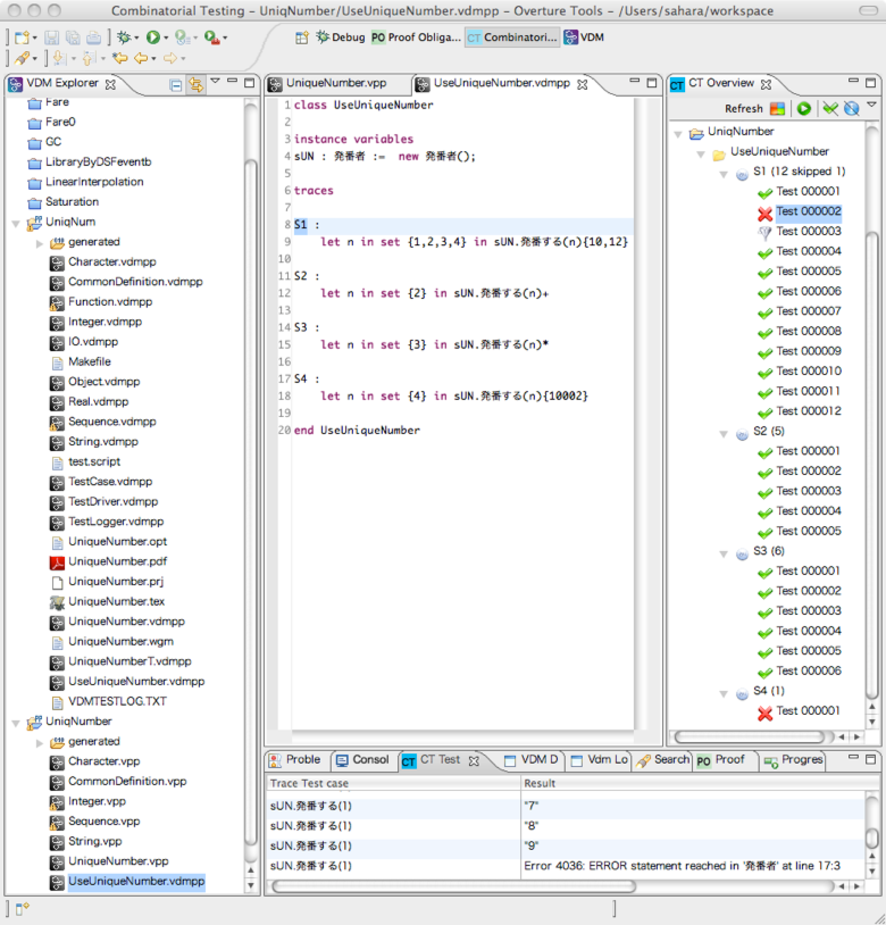
\includegraphics[width=55zw, keepaspectratio]{./UniqNumber/image/CombinatorialTestScreen.pdf}}
	\caption{組合せテスト実行画面例}
	\label{fig:CombinatorialTestScreen}
	\index{くみあわせてすとじっこうがめんれい@組合せテスト実行画面例}
\end{figure}

図\ref{fig:CombinatorialTestScreen}右上のCT Overviewサブ・ウィンドウに組合せテストの実行結果が表示されている。

テストS1の最初のテストTest 000001は正常終了したので、緑色のチェックマークが付く。
もちろん、正常終了したからといって、このテストケースが正しいとは限らない。
不変条件、事前条件、事後条件が正しく記述されている場合は意味的にも正しいが、
それ以外の場合は、単に実行が正常に終了したことを示すだけであって、
意図した結果が得られているとは限らないので、注意が必要である。

次の、Test 000002は実行時エラーがあったことを示して、赤色の×マークが付いている。
このエラー原因は、右下のCT Testサブ・ウィンドウに示されていて、
発番者クラス17行目第3カラムでERROR文が実行されたことが示されている。
ERROR文は、エラーがあったことを示して停止するだけなので、
エラー原因は発番者クラスのVDM++ソースを見て判断しなければならない
\footnote{エラー原因を表示するようにVDM++仕様を作成することは、例外処理文などを使えば可能である。
ここでは、説明の単純化のためにERROR文を使った}。

Test 000003は、Test 000002と同じ順序でテストケースを実行するため、
必ず同じ所でエラーとなるので、それを検知した組合せテストケース機能が、
実行せずにエラーを表示している。この印が漏斗のような灰色のアイコンである。

組合せテストは、このようにして、数千件のテストケースを実行できるので、
複雑な組合せ条件をテストするのに適している。


\subsection{回帰テスト}
	\label{RegressionTest}
	\index{かいきてすと@回帰テスト}

	回帰テスト(regression test)は、ソフトウェアが退化していないか確認するテストである。
	テストケースと期待する結果を一体にして記述し、実行して一致するか確認する。

	VDM++では、VDMUnitと呼ばれる回帰テスト用ライブラリを使用して回帰テストを行う。

	回帰テスト実行用のクラスは\ref{RegressionTestExecute}節のTestAppクラスを参照していただきたい。
	回帰テストケースは、\ref{RegressionTestcase}節の回帰テストケースクラスと、そのサブクラス群を参照していただきたい。

	回帰テストのノーマルケースの例は、\ref{RegressionTestNormalCase}節のTestCaseT0001クラスを参照のこと。
	回帰テストのエラーケースの例は、\ref{RegressionTestErrorCase}節のTestCaseT0003クラスを参照のこと。


\section{プログラミング}
	\label{Programming}
	\index{ぷろぐらみんぐ@プログラミング}

	VDM++仕様を見ながら、以下の作業を行った。

	\begin{itemize}
	\item 実装用フレームワークを作成
	\item VDM++仕様を見て、手作業でプログラム作成 \\
		VDM++からC++生成も可能だが
		\begin{itemize}
		\item 独自のミドルウェアに合わせて調整する時間的余裕が無かった(日本フィッツ事例)。 \\
					生成されるプログラムの性能は、恐らく問題ないと予想したが
						\footnote{SCSKでは、現在、コード生成機能を大幅に改良し、
							エンタープライズシステム用Java生成フレームワークを試作中。}、
					プロジェクト工数の5\%程度の作業に時間を取られたくなかったため、
					プログラム生成は使用しなかった。
		\item 生成されたC++プログラムの性能が、十分でなかった(フェリカネットワークス事例)。
		\end{itemize} 
	\item 単純な画面生成プログラムを作成し、GUI生成(日本フィッツ事例)。
	\item オランダの花市場オークションシステム事例では
		\index{おらんだのはなしじょうオークションしすてむ@オランダの花市場オークションシステム事例}
		1999年にC++生成を利用し、ソースの90\%を生成。残りは、手でコーディング。
	\end{itemize} 

\section{プログラムのテスト}
	\label{TestOfProgram}
	\index{ぷろぐらむのてすと@プログラムのテスト}

	プログラムのテストは以下のように行った。

	\begin{itemize}
	\item 単体テスト
		\index{たんたいてすと@単体テスト}
		\begin{itemize}
		\item Purify
				\footnote{現在の製品名は、Rational PurifyPlus。
					\url{http://www-06.ibm.com/software/jp/rational/products/purifyp/highlights.html}}
				でソースの静的チェック \\
				メモリの破壊可能性などをチェックした。
		\item C++コードカバレージ機能でテスト達成率測定
			\begin{itemize}
			\item Excelデータからテストケースを生成する簡単なプログラムを作成 \\
				メモリの破壊可能性などをチェックした。
			\item VDM++テストケースを、C++プログラムのExcelの単体テストケースに手作業で変換 \\
				C0レベルで98\%カバー
			\end{itemize} 
		\item 仕様エミュレータを内蔵(フェリカネットワークス事例) \\
				実装に対し、ランダムにコマンドを送信し、応答が正しいか確認(フェリカネットワークス事例)
		\end{itemize} 
	\item 連結テスト \\
		要求定義担当者が、業務知識とWordで作成したユースケースから、テストケース生成(日本フィッツ事例)
	\item 総合テスト
		\index{そうごうてすと@総合テスト}
		\begin{itemize}
		\item 評価環境を構築(フェリカネットワークス事例) \\
			ICチップファームウェアと、実装と、形式仕様とが、同様の動作をすることを確認。
		\item VDM仕様に基づいて、ランダム評価ツールを作成し、数億件のテストケースを生成し、
			動的チェック(フェリカネットワークス事例)
		\item 業務専門家全員で総合テストケース作成 (日本フィッツ事例)
		\end{itemize} 
	\end{itemize} 

\section{開発管理}
	\label{DevelopmentManagement}
	\index{かいはつかんり@開発管理}

	開発管理は、開発時点で実用性があると分かっていたソフトウェア工学技術とツールを使用して、
	以下のように行った。

	\begin{itemize}
	\item 版管理ツールcvsを使用 \\
			\index{はんかんりつーる@版管理ツール}
			VDM++仕様、ソースプログラム、Wordなどのドキュメント、テストケース、
			プログラム実行モジュールなど、全てのリソースを版管理した。
	\item Swiki(Squeak Wiki)サーバーを使って、共同作業を円滑にした(日本フィッツ事例)。
	\item ISO\,9000にしたがって、単体テスト以後の全欠陥をnotesで記録し、追跡した (日本フィッツ事例)。
	\end{itemize} 

\section{開発体制}
	\label{DevelopmentTeamStructure}
	\index{かいはつたいせい@開発体制}

\subsection{日本フィッツの開発体制}
	\index{にほんふぃっつのかいはつたいせい@日本フィッツの開発体制}

	仕様作成チーム、実装チーム、証券業務専門家チームの間で、相互チェックを行いながら開発を行った。

	証券業務専門家チームは、ユースケースの最初の案をWordで作成し、VDM++仕様の回帰テスト結果を主としてチェックした。
	VDM++ソースのチェックは、計算式部分など一部のみ行った。
	テスト工程では、連結テスト、総合テストのテストケース作成と結果の確認を行った。

	仕様作成チームは、Wordで記述されたユースケース相当の仕様をチェックしながら、
	VDM++では、ほぼ完全にそれらを書き換えた。
	プログラムの単体テスト工程では、実装チームの作成したテストケースとVDM++仕様のテストケースを目で比較し、
	不足しているテストケースを追加した。

	実装チームは、VDM++仕様を全て読み、手作業でプログラムに変換した。
	他チームの成果物のほとんどをレビューし、チェックした。
	

\subsection{フェリカネットワークスの開発体制}
	\index{ふぇりかねっとわーくすのかいはつたいせい@フェリカネットワークスの開発体制}

	仕様作成チーム、評価チーム、実装チームの間で、相互チェックを行いながら開発を行った。

	各チームの相互チェックの様子を、図\ref{fig:FeliCaTeamStructure}に示す。

\begin{figure}[h]
	\centering
	{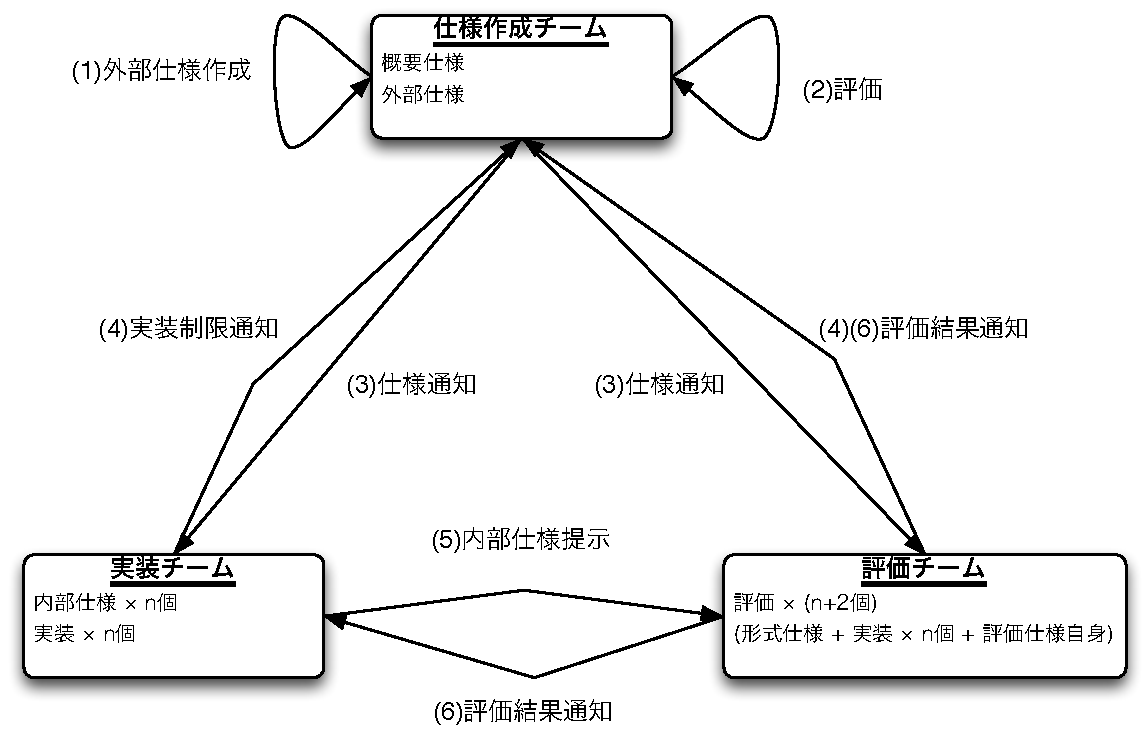
\includegraphics[width=55zw, keepaspectratio]{./Chapter4/image/FeliCaTeam.pdf}}
	\caption{フェリカネットワークスの開発体制}
	\label{fig:FeliCaTeamStructure}
	\index{ふぇりかねっとわーくすのかいはつたいせい@フェリカネットワークスの開発体制}
\end{figure}

\begin{enumerate}
	\item 仕様作成チームは、日本語の概要仕様からVDM++による外部仕様を作成し、
	\item 回帰テストを行って、外部仕様の評価(正当性検証と仕様作成チームの観点からの妥当性確認)を行い、
	\item 評価チームと実装チームに評価済みの仕様を通知する。
	\item 評価チームは、評価チームの評価結果を仕様作成チームにフィードバックし、\\
		実装チームは、内部仕様と実装を通して発見した、実装上の制限を仕様作成チームにフィードバックする。
	\item 実装チームは、作成した内部仕様を評価チームに提示し、
	\item 評価チームは、VDM++による形式仕様と、n個のチップの実装仕様と、評価仕様自身を総合して評価し、\\
		実装チームおよび仕様作成チームに評価結果をフィードバックする。
\end{enumerate}

	
